\documentclass{beamer}
\usepackage{caption}
\usepackage{listings}
\usepackage{tabularx}
\usepackage{graphicx}
\usepackage{tikz}
\usepackage{booktabs}
\usepackage{pgfplotstable}
\usetikzlibrary{chains,shapes,arrows,positioning,backgrounds}
\pgfplotsset{compat=1.14}

\title{Binary Code Translation from Register to Stack based code}
\author{Charles Pigott}
\institute{Computer Science Dept\\ University of York}
\date{May 2017}

\setbeamerfont{caption}{size=\scriptsize}
\DeclareCaptionLabelFormat{nonum}{#1}
\captionsetup[lstlisting]{font={scriptsize},labelformat=nonum}
\lstset{basicstyle=\Tiny\ttfamily,captionpos=b}

\resetcounteronoverlays{lstlisting}

\newcolumntype{L}{>{\scriptsize\ttfamily\arraybackslash}p{3.5em}}

\begin{document}

\frame{\titlepage}

\begin{frame}
  \frametitle{Introduction}

  \begin{figure}
    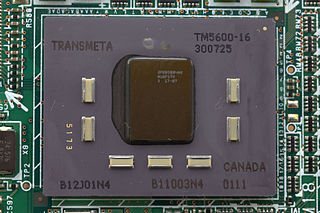
\includegraphics[width=0.3\textwidth]{imgs/Transmeta_TM5600}
    \caption{The Transmeta TM5600 CPU from a Fujitsu laptop}
  \end{figure}
\end{frame}

\begin{frame}
  \frametitle{Register machines}
   \begin{columns}
     \column{0.6\linewidth}
       \begin{itemize}
         \item<1-> Named locations
         \item<2-> Almost exclusively used in practice
         \item<3-> RISC \& CISC
       \end{itemize}
     \column{0.4\linewidth}
       \begin{figure}
         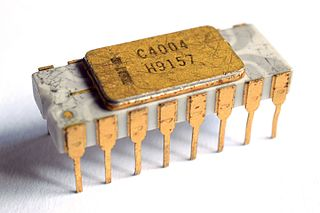
\includegraphics[width=\linewidth]{imgs/Intel_C4004}
         \caption{Intel's 4004 microprocessor}
       \end{figure}
   \end{columns}
\end{frame}

\begin{frame}[fragile]
  \frametitle{Stack machines}
  \begin{columns}
    \column{0.5\linewidth}
    \begin{itemize}
      \item<1-> Stack instead of registers
      \item<2-> Comparatively simpler than register architectures
      \item<3-> Hardly used in production these days
    \end{itemize}
    \column{0.5\linewidth}

    \begin{lstlisting}[caption={8 Queens problem in Forth}]
: .sol3 ( fn ... f1 x x f0 -- unchanged )
 dup N 0 do
   I 3 * 4 + pick ( fi fi+1 )
   2dup xor .rank  nip
 loop drop cr ;
: third ( a b c -- a b c a ) 2 pick ;    \ >r over r> swap ;
: poss ( a b c -- a b c a&b&c ) dup 2over and and ;
: next3 ( dl dr f Qfilebit -- dl dr f dl' dr' f' )
 invert >r third r@ and 2* 1+  third r@ and 2/  third r> and ;
\ bitmasks for unused diagonals and files
: try ( dl dr f -- )
 dup if 1 nodes +!  poss
   begin ?dup while
     dup >r lowBit next3 recurse r> lowBit-
   repeat
 else ( .sol3) 1 solutions +! then drop 2drop ;
: queens3  -1 dup Nbits try ;
    \end{lstlisting}
  \end{columns}
\end{frame}

\begin{frame}[fragile]
  \frametitle{Stack optimisations}
  \begin{columns}
    \column{0.65\linewidth}
    \begin{itemize}
      \item<1-> Peephole (McKeeman, 1965)
      \item<2-> Stack scheduling (Koopman, 1995)
      \item<3-> Inter-block scheduling (Bailey, 2000)
      \item<4-> Global scheduling (Shannon, 2006)
    \end{itemize}
    \column{0.35\linewidth}
    \only<1>{%
      \noindent\begin{table}
      \begin{tabularx}{\linewidth}{L L}
        \normalfont{Original stack code} &
        \normalfont{Optimised stack code} \\ \toprule
      SET 1\newline
      ADD
      &
      INC \\ \midrule
      SET 0\newline
      TEQ\newline
      DROP
      &
      TSZ \\ \midrule
      DUP\newline
      SWAP
      &
      DUP \\ \midrule
      SET x\newline
      DROP
      &
      <NOP> \\ \bottomrule
      \end{tabularx}
      \caption{Peephole optimisation examples}
      \end{table}
    }
  \end{columns}
\end{frame}

\begin{frame}
  \frametitle{Binary translation}
  \begin{itemize}
    \item Transputer
    \item IBM
  \end{itemize}
\end{frame}

\begin{frame}
  \frametitle{Binary translation}
  \framesubtitle{Transmeta}
  \begin{columns}
    \column{0.35\linewidth}
    \begin{itemize}
      \item<1-> Published 2000
      \item<2-> Sophisticated x86 translation and emulator
    \end{itemize}
    \column{0.65\linewidth}
  \begin{figure}
    \scalebox{0.5}{%
    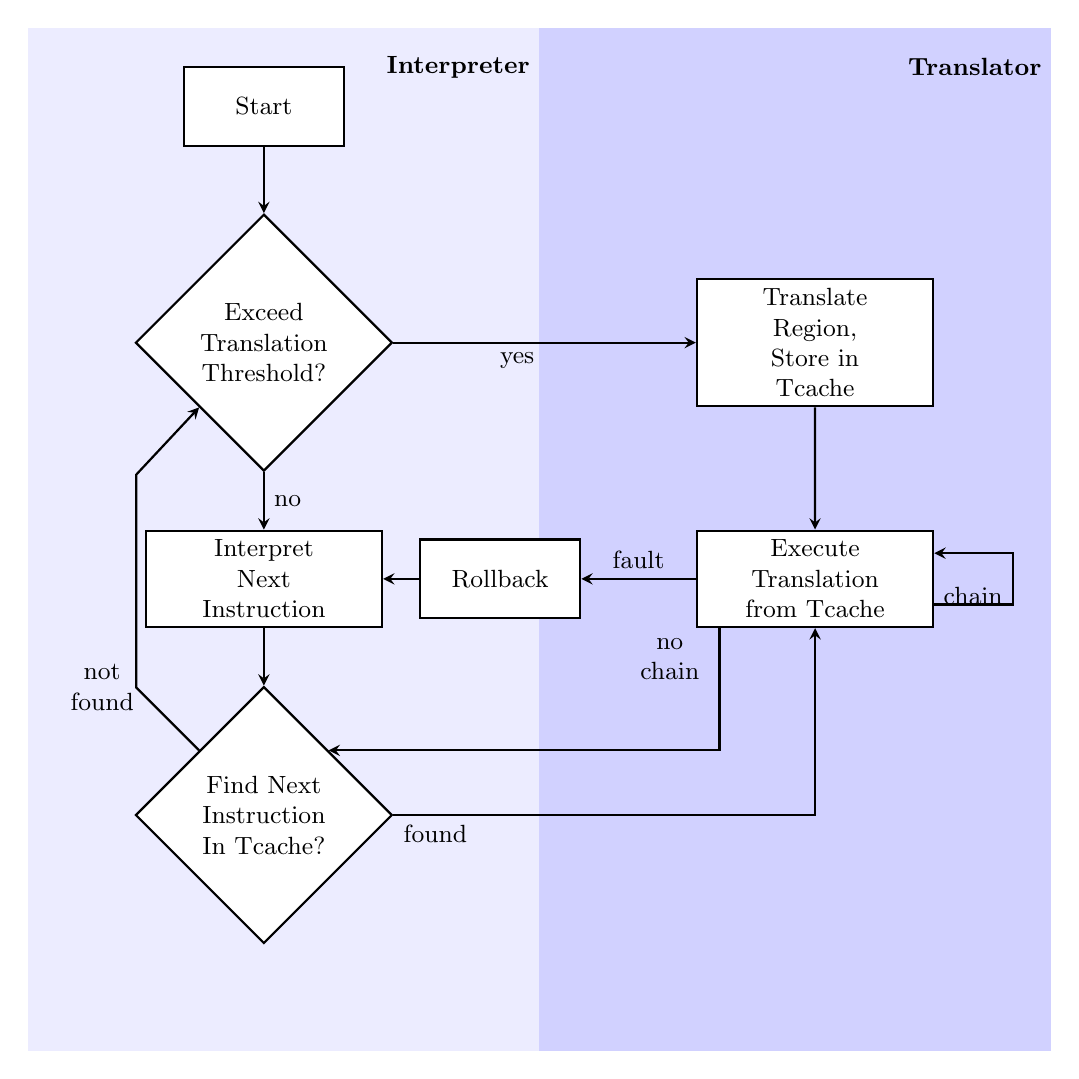
\begin{tikzpicture}[node distance=3cm, on grid, auto, >=stealth, thick,
                        text centered, font=\small]
      \tikzstyle{process} = [rectangle, minimum width=3cm, minimum height=1cm,
                             draw=black, fill=white, text width=1.8cm]
      \tikzstyle{decision} = [diamond, minimum width=3cm, minimum height=1cm,
                              draw=black, fill=white, text width=1.8cm]

      \begin{scope}[on background layer]
        \fill[blue!25!,opacity=.3] (-3, 1) rectangle (3.5, -12);
        \fill[blue!60!,opacity=.3] (3.5, 1) rectangle (10,-12);
        \node[left] at (3.5,.5) {\textbf{Interpreter}};
        \node[left] at (10,.5) {\textbf{Translator}};
      \end{scope}

      \node (start) [process, minimum width=2cm]{Start};
      \node (dec1)  [decision, below=of start] {Exceed Translation Threshold?};
      \node (pro1)  [process, right=of dec1, xshift=4cm] {Translate Region, Store in Tcache};
      \node (pro4)  [process, below=of dec1]  {Interpret Next Instruction};
      \node (pro3)  [process, right=of pro4,minimum width=2cm]  {Rollback};
      \node (pro2)  [process, right=of pro3, xshift=1cm] {Execute Translation from Tcache};
      \node (dec2)  [decision, below=of pro4] {Find Next Instruction In Tcache?};

      \draw [->] (start) -- (dec1);
      \draw [->] (dec1) -- node[anchor=north east] {yes} (pro1);
      \draw [->] (dec1) -- node {no} (pro4);
      \draw [->] (pro1) -- (pro2);
      \draw [->] (pro4) -- (dec2);
      \draw [->] (pro3) -- (pro4);
      \draw [->] (pro2) -- node[anchor=south] {fault} (pro3);
      \draw [->] ([yshift=3mm] pro2.south east) |- ++(1, 0) |-
      node[yshift=-3mm, anchor=north east] {chain} ([yshift=-3mm] pro2.north east);
      \draw [->] ([xshift=3mm] pro2.south west) node[anchor=north east, text width=1cm]
      {no chain} |- (dec2.north east);
      \draw [->] (dec2.east) node[anchor=north west] {found} -| (pro2.south);
      \draw [->] (dec2.north west) -- ++(-0.8, 0.8) node[anchor=east,
      text width=1cm,xshift=2mm] {not found} -- ++(0, 2.7) -- (dec1.south west);
    \end{tikzpicture}
    }
    \caption{Typical CMS Control Flow}
  \end{figure}

  \end{columns}
\end{frame}

\begin{frame}
\frametitle{Implementation}
  \begin{columns}
    \column{0.5\linewidth}
  \begin{itemize}
    \item<1-> Implemented in C++
    \item<2-> Source register architecture DCPU-16
    \item<3-> Target stack architecture J5
    \item<4-> Implemented Peephole \& Koopman-style optimisations
    \item<5-> Implemented basic translation cache
    \item<6-> Tested using 4 different register test programs
  \end{itemize}
  \column{0.5\linewidth}
    \only<7>{%
\begin{figure}
  \scalebox{0.4}{%
  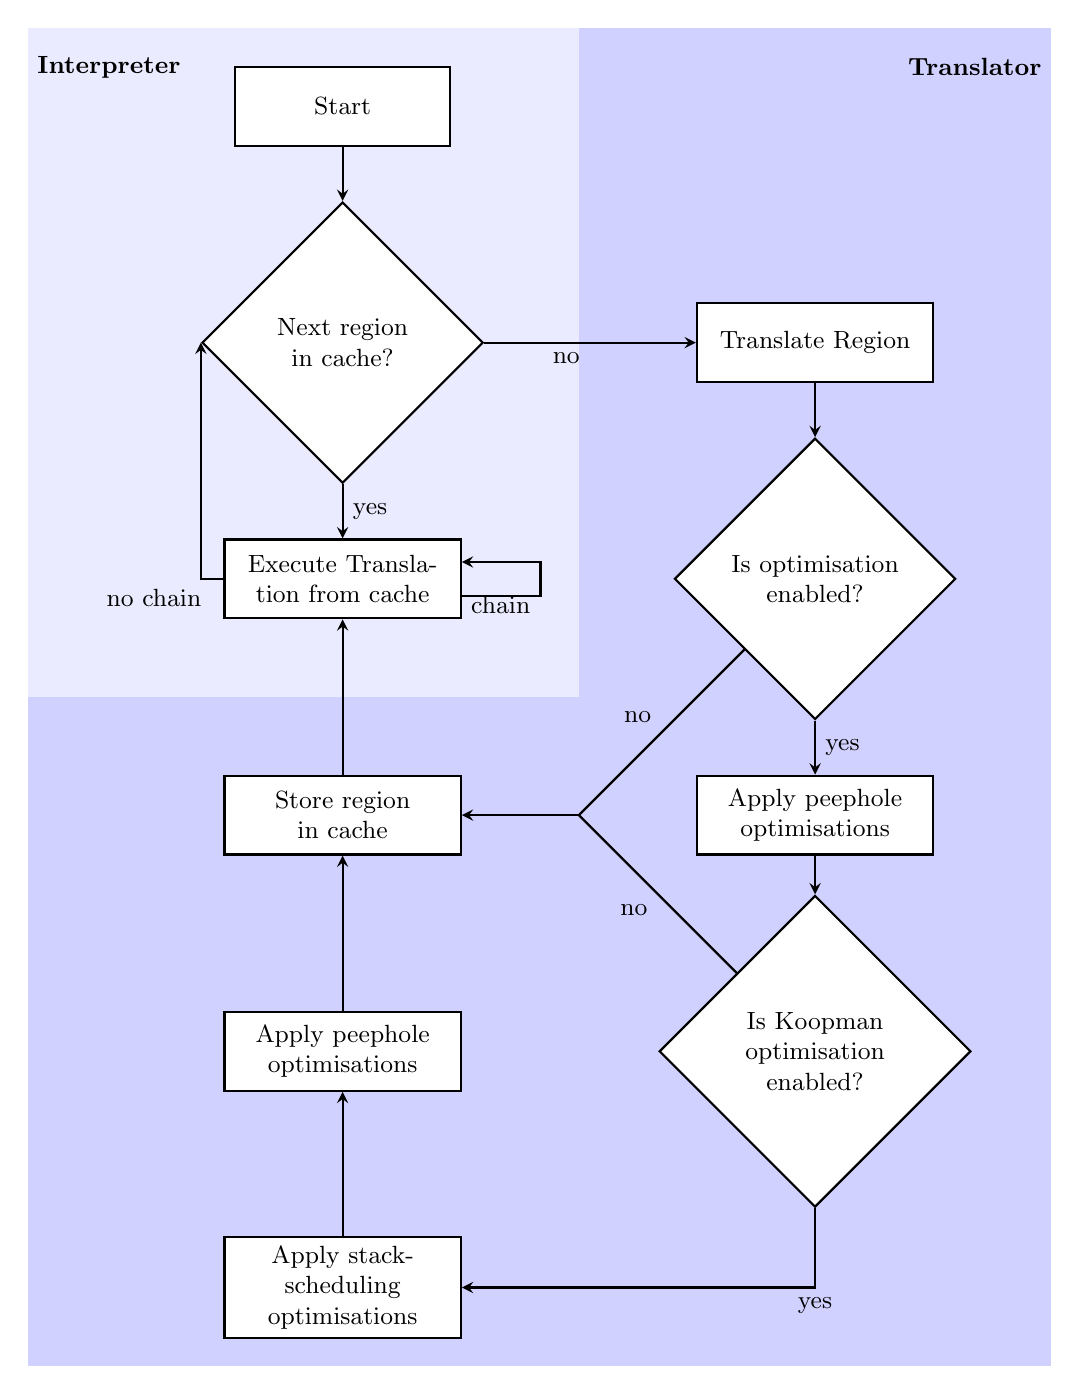
\begin{tikzpicture}[node distance=3cm, on grid, auto, >=stealth, thick,
                      text centered, font=\small]
    \tikzstyle{process} = [rectangle, minimum width=3cm, minimum height=1cm,
                           draw=black, fill=white, text width=2.5cm]
    \tikzstyle{decision} = [diamond, minimum width=3cm, minimum height=1cm,
                            draw=black, fill=white, text width=2.5cm]

    \begin{scope}[on background layer]
      \fill[blue!60!,opacity=.3] (-4, 1) rectangle (9,-16);
      \fill[white] (-4, 1) rectangle (3, -7.5);
      \fill[blue!25!,opacity=.3] (-4, 1) rectangle (3, -7.5);
      \node[right] at (-4,.5) {\textbf{Interpreter}};
      \node[left] at (9,.5) {\textbf{Translator}};
    \end{scope}

    \node (start) [process, minimum width=2cm] {Start};
    \node (dec1)  [decision, below=of start] {Next region in cache?};
    \node (pro1)  [process, right=of dec1, xshift=3cm] {Translate Region};
    \node (pro2)  [process, below=of dec1] {Execute Translation from cache};
    \node (dec2)  [decision, below=of pro1] {Is optimisation\allowbreak enabled?};
    \node (pro3)  [process, below=of dec2] {Apply peephole\allowbreak optimisations};
    \node (dec3)  [decision, below=of pro3] {Is Koopman optimisation enabled?};
    \node (pro6)  [process, below=of pro2] {Store region in cache};
    \node (pro5)  [process, below=of pro6] {Apply peephole\allowbreak optimisations};
    \node (pro4)  [process, below=of pro5] {Apply stack-scheduling\allowbreak optimisations};
    \coordinate[right=of pro6] (invis);

    \draw [->] (start) -- (dec1);
    \draw [->] (dec1) -- node[anchor=north east] {no} (pro1);
    \draw [->] (dec1) -- node {yes} (pro2);
    \draw [->] (pro1) -- (dec2);
    \draw [->] (dec2) -- node {yes} (pro3);
    \draw [->] (invis) -- (pro6);
    \draw (dec2.south west) -- node[anchor=south east] {no} (invis);
    \draw (dec3.north west) -- node[anchor=north east] {no} (invis);
    \draw [->] (pro3) -- (dec3);
    \draw [->] (dec3) |- node {yes} (pro4);
    \draw [->] (pro4) -- (pro5);
    \draw [->] (pro5) -- (pro6);
    \draw [->] (pro6) -- (pro2);
    \draw [->] ([yshift=3mm] pro2.south east) |- ++(1, 0) |-
    node[yshift=-3mm, anchor=north east] {chain} ([yshift=-3mm] pro2.north east);
    \draw [->] (pro2.west) node[anchor=north east, text width=1.5cm] {no chain} -| (dec1.west);
  \end{tikzpicture}
  }
  \caption{Implementation structure}\label{fig:implementationstructure}
\end{figure}
    }
  \end{columns}
\end{frame}

\pgfplotstableread[col sep=comma,header=false]{%
bsort,24024,22343,22233
fib20,665,608,606
primes,6717,6619,6619
tri100,111381,106332,106332
}\tracedata%

\pgfplotstableread[col sep=comma,header=false]{%
bsort,7792,6703,6065
fib20,234,196,175
primes,1912,1912,1643
tri100,35345,35345,30296
}\tracememdata%

\pgfplotsset{%
  relative series/.style={%
    table/y expr=\thisrow{#1}/\thisrow{1},
    table/meta=#1
  },
  relative graph/.style={%
    width=13cm,
    ymajorgrids=true,
    major x tick style = transparent,
    major y tick style = transparent,
    scaled y ticks = false,
    ybar=0pt,
    ymin=0.5,
    bar width=0.75cm,
    enlarge x limits=0.2,
    symbolic x coords={bsort,fib20,primes,tri100},
    xtick=data,
    legend cell align=left,
    legend style={%
      at={(1,0)},
      anchor=south west,
      column sep=1ex
    }
  }
}

\begin{frame}
\frametitle{Results}
\framesubtitle{Traces}
\begin{figure}
    \scalebox{0.5}{%
  \begin{tikzpicture}
    \begin{axis}[relative graph]
      \addplot table [relative series=1] {\tracedata};
      \addplot table [relative series=2] {\tracedata};
      \addplot table [relative series=3] {\tracedata};
      \legend{Base,Peephole,Koopman}
    \end{axis}
  \end{tikzpicture}
  }
  \caption{Relative no.\ of instructions executed}\label{fig:relativeinstructions}
\end{figure}
\end{frame}

\begin{frame}
\frametitle{Results}
\framesubtitle{Traces}
\begin{figure}
    \scalebox{0.5}{%
  \begin{tikzpicture}
    \begin{axis}[relative graph]
      \addplot table [relative series=1] {\tracememdata};
      \addplot table [relative series=2] {\tracememdata};
      \addplot table [relative series=3] {\tracememdata};
      \legend{Base,Peephole,Koopman}
    \end{axis}
  \end{tikzpicture}
  }
  \caption{Relative no.\ of LOAD/STORE instructions executed}\label{fig:relativememinstructions}
\end{figure}
\end{frame}

\pgfplotstableread[col sep=comma]{%
Register,Stack,Peephole,Koopman
%34,103,102,102
2,9,8,8
5,25,24,24
3,24,24,23
6,27,25,25
4,22,21,21
6,34,32,32
7,20,20,18
2,6,6,6
2,12,12,12
4,17,16,16
3,17,17,17
4,24,24,24
2,6,6,6
2,6,6,6
4,20,19,19
4,23,22,22
}\blockdata%

\pgfplotstableread[col sep=comma]{%
Register,Stack,Peephole,Koopman
%34,35,34,34
2,3,3,3
5,8,7,6
3,10,10,9
6,6,5,5
4,6,6,5
6,6,6,4
7,12,11,9
2,2,6,2
2,2,2,2
4,4,5,3
3,5,4,5
4,7,7,6
2,2,2,2
2,2,2,2
4,7,7,6
4,5,5,4
}\blockmemdata%

\begin{frame}
\frametitle{Results}
\begin{columns}
  \column{0.5\linewidth}
  \begin{figure}
    \scalebox{0.5}{%
      \begin{tikzpicture}
        \begin{axis}[
            xlabel=No.\ of register instructions,
          ylabel=No.\ of stack instructions,
          legend cell align=left,
          legend style={%
            at={(1,0)},
          anchor=south west,
          column sep=1ex
          }
        ]
          \addplot [only marks,mark=x,blue] table [y=Stack] {\blockdata};
          \addplot [thick,blue] table [y={create col/linear regression={y=Stack}}] {\blockdata};
          \addlegendentry{Base}
          \addplot [only marks,mark=x,red] table [y=Peephole] {\blockdata};
          \addplot [thick,red] table [y={create col/linear regression={y=Peephole}}] {\blockdata};
          \addlegendentry{Peephole}
          \addplot [only marks,mark=x,brown] table [y=Koopman] {\blockdata};
          \addplot [thick,brown] table [y={create col/linear regression={y=Koopman}}] {\blockdata};
          \addlegendentry{Koopman}
          \legend{Base,,Peephole,,Koopman}
        \end{axis}
      \end{tikzpicture}
    }
    \caption{Register blocks to stack equivalents}
  \end{figure}
  \column{0.5\linewidth}

  \begin{figure}
    \scalebox{0.5}{%
      \begin{tikzpicture}
        \begin{axis}[
            xlabel=No.\ of register instructions,
          ylabel=No.\ of LOAD/STORE stack instructions,
          legend cell align=left,
          legend style={%
            at={(1,0)},
          anchor=south west,
          column sep=1ex
          }
        ]
          \addplot [only marks,mark=x,blue] table [y=Stack] {\blockmemdata};
          \addplot [thick,blue] table [y={create col/linear regression={y=Stack}}]
          {\blockmemdata};
          \addlegendentry{Base}
          \addplot [only marks,mark=x,red] table [y=Peephole] {\blockmemdata};
          \addplot [thick,red] table [y={create col/linear regression={y=Peephole}}]
          {\blockmemdata};
          \addlegendentry{Peephole}
          \addplot [only marks,mark=x,brown] table [y=Koopman] {\blockmemdata};
          \addplot [thick,brown] table [y={create col/linear regression={y=Koopman}}]
          {\blockmemdata};
          \addlegendentry{Koopman}
          \legend{Base,,Peephole,,Koopman}
        \end{axis}
      \end{tikzpicture}
    }
    \caption{Register blocks to stack memory read/writes}
  \end{figure}
\end{columns}
\end{frame}

\pgfplotstableread[col sep=comma,header=false]{%
bsort,97292,93746,92454,40902,37356,36064
fib20,1300,1224,1142,1300,1224,1142
primes,19615,19516,18978,11981,11882,11344
tri100,202089,197040,186942,192583,187534,177436
}\costdata%

\begin{frame}
  \frametitle{Results}
\begin{figure}
  \scalebox{0.5}{%
  \begin{tikzpicture}
    \begin{axis}[relative graph,bar width=0.4cm,ymin=0,width=15cm]
      \addplot table [relative series=1] {\costdata};
      \addplot table [relative series=4] {\costdata};
      \addplot table [relative series=2] {\costdata};
      \addplot table [relative series=5] {\costdata};
      \addplot table [relative series=3] {\costdata};
      \addplot table [relative series=6] {\costdata};
      \legend{Base,Base Cached,Peephole,Peephole Cached,Koopman,Koopman Cached}
    \end{axis}
  \end{tikzpicture}
  }
  \caption{Relative program cost with and without caching}\label{fig:progcost}
\end{figure}
\end{frame}

\begin{frame}
\frametitle{Conclusions}
\framesubtitle{Further work}
  \begin{itemize}
    \item<1-> Further optimisation algorithms
    \item<2-> More sophisticated caching system
    \item<3-> More formal testing
  \end{itemize}
\end{frame}
\begin{frame}
  \frametitle{Conclusions}
  \centering
  \Large{Any questions?}
\end{frame}

\end{document}

